\documentclass[a4paper,titlepage]{article}

% use this when images are included
\usepackage{float}
\usepackage{graphicx}
\graphicspath{ {./images/} }

% use for lines of code
\usepackage{listings}

% use for links, also links list of contents
\usepackage{hyperref}


\title{Digital Pen}
\date{2021\\ June}
\author{Max-Felix Müller\\ \\ 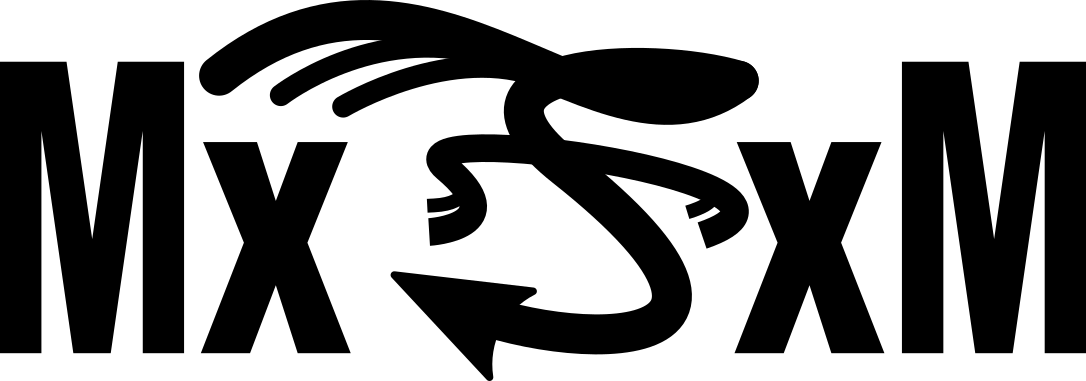
\includegraphics[width=\textwidth]{mxfxm.png}}

\begin{document}
\maketitle
\tableofcontents
\newpage
\listoffigures %delete if not necessary
\listoftables %delete if not necessary
\newpage

\section*{Abstract}

Using the Tiny Motion Trainer and an Arduino Nano 33 BLE Sense, a digital pen was created.

The digital pen can be used to draw letters into the air.
A neural network running on the microcontroller itself will predict which letter was drawn.
The accelerometer and gyroscope data is used for the prediction.

All letters can be detected with over 50\% certainty.
By modifying the example output of the Tiny Motion Trainer the model can be executed standalone.

An additionaly battery, charging and protection circuit could be added to make the pen truly wireless.

\newpage
\section{Inspiration}

What originally inspired this project was the video from Zack Freedman about his data glove.
The data glove is a glove with a motion sensor and a Teensy microcontroller.

It is nice that the glove also detects gestures, by measuring which fingers are extended.
That way the hand motion can be interpreted differently, for example to differentiate between a mouse and a keyboard interface.

However, the glove has to be worn and especially in hot summer days, this might not be preferable.

\section{First Section}
This is the first section.

\subsection{A Subsection}
Some maths. \\

$R_{1} = R_{2} = Z_{0} * \frac{N + 1}{N - 1} $\\

$R_{3} = Z_{0} * \frac{N^2 - 1}{2N} $\\

\subsection{Second Subsection}

With images...

\begin{figure}[H]
    %\includegraphics[width=\textwidth]{filename.png}
    \caption{Title of the image}
\end{figure}

\subsubsection{Subsub Section}
A line of code:

\begin{lstlisting}
    dump_errors(odrv0, True)
\end{lstlisting}

\newpage
\section{Links}

Ressources used for an in this project: \\

The video from Zack Freedman \\
\href{https://www.youtube.com/watch?v=6raRftH9yxM}{https://www.youtube.com/watch?v=6raRftH9yxM} \\

\end{document}
